\documentclass{article}

\usepackage{a4wide}
\usepackage[utf8]{inputenc}
\usepackage[T1]{fontenc}
\usepackage[french]{babel}
\usepackage[babel=true]{csquotes} % guillemets français
\usepackage{graphicx}
\graphicspath{{Images/}}
\usepackage{color}
\usepackage{hyperref}
\hypersetup{colorlinks,linkcolor=,urlcolor=blue}

\usepackage{amsmath}
\usepackage{amssymb}


\title{UnivMap}
\author{Damien LAOUSSING, Dylan CHERRIER, L3 informatique}
\date{\today}

\begin{document}

\maketitle %% pour écrire le titre


%% Le résumé:
\begin{abstract}
  UnivMap est une application mobile iOS et Android destinée au nouveau
  étudiant afin de les aider à se repérer au sein de l'Université de la Réunion.
\end{abstract}


\section{Introduction}
\label{section:intro} % pour faire référence à la section ailleurs (\ref{...} voir plus bas)

Hello World!


\section{Description générale de l'application}
Voici une belle capture d'écran d'une partie en cours:
\begin{center}
  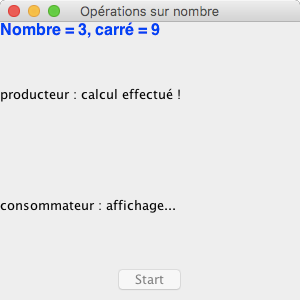
\includegraphics[scale=0.5]{exo3_1_1.png}
\end{center}

Une liste à \textbf{puces}:
\begin{itemize}
\item la documentation d'\textit{Android}~\cite{androidDoc}
  est bien écrite,
\item celle d'\textit{iOS}~\cite{iosDoc} aussi!
\end{itemize}
% \cite{...} permet de faire référence à des éléments de la
% bibliographie.

Une liste numérotée:
\begin{enumerate}
\item premier item
\item second item
\end{enumerate}



\section{Architecture du code}
% \ref{...} permet de faire référence à un élément défini
% ailleurs dans le document (voir \label{...} plus haut).
Contrairement à la section~\ref{section:intro},
moi je dis: \textit{Coucou!}

\subsection{Android} %% une sous-section
Pour écrire du code, on peut par exemple utiliser l'environnement
\textit{verbatim}:
\begin{verbatim}
public class Main {
   public static void main(String[] args) {
      System.out.println("Hello World!");
   }
}
\end{verbatim}

\subsection{iOS} %% une autre sous-section


\section{Quelques points délicats/intéressants}


\section{Conclusion}


%%% La bibliographie:
\bibliographystyle{plain}
\bibliography{ma_biblio}

\end{document}
